\usetikzlibrary{calc}
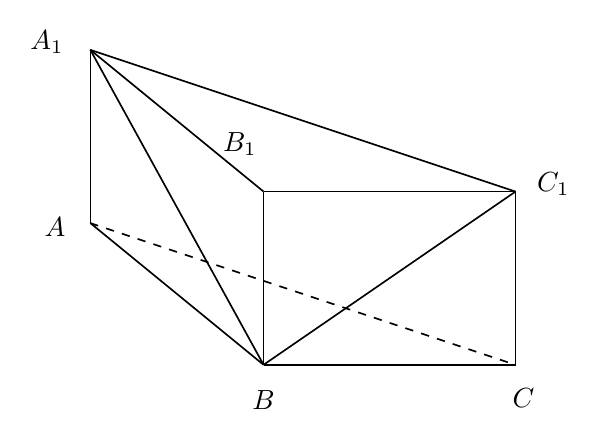
\begin{tikzpicture}[x=1cm,y=1cm,line width=0.6pt,color=black,font=\normalsize]
% Right triangular prism A1B1C1-ABC, vertical lateral edges
\coordinate (A) at (0,2.0);
\coordinate (B) at (2.2,0.2);
\coordinate (C) at (5.4,0.2);
\coordinate (Aone) at (0,4.2);
\coordinate (Bone) at (2.2,2.4);
\coordinate (Cone) at (5.4,2.4);
% bottom triangle
\draw[dashed] (A)--(C);
\draw[solid] (A)--(B);
\draw[solid] (B)--(C);
% vertical edges
\draw[solid] (A)--(Aone);
\draw[solid] (B)--(Bone);
\draw[solid] (C)--(Cone);
% top triangle
\draw[solid] (Aone)--(Bone);
\draw[solid] (Bone)--(Cone);
\draw[solid] (Aone)--(Cone);
% tetrahedron A1-B-C1 faces
\draw[solid] (Aone)--(B);
\draw[solid] (B)--(Cone);
% labels with clearance
\node[inner sep=1pt] at ($(Aone)+(-0.55,0.10)$) {$A_{1}$};
\node[inner sep=1pt] at ($(A)+(-0.45,-0.05)$) {$A$};
\node[inner sep=1pt] at ($(Bone)+(-0.30,0.60)$) {$B_{1}$};
\node[inner sep=1pt] at ($(B)+(0.0,-0.45)$) {$B$};
\node[inner sep=1pt] at ($(Cone)+(0.48,0.10)$) {$C_{1}$};
\node[inner sep=1pt] at ($(C)+(0.10,-0.42)$) {$C$};
\end{tikzpicture}
